\chapter{Optimization}\label{section:optimization}

With the model of farm/turbine power established, the following section treats the embedding of the trained model(s)  into a stochastic optimization problem. The underlying theory of optimization under uncertainty and constraint learning is introduced before the actual optimization problems are defined, required models trained and results discussed.

\section{Optimization under Uncertainty}

TODO : REWRITE FIRST SCENTENCE

While some things in life are certain, most are not and this is as true for optimization as for anything else. That means, that while optimizing anything from next year's crop to tomorrow's energy pricing might be done by assuming fixed values for the parameters of an optimization problem, in reality, most of these parameters contain uncertainty. The field of Stochastic Programming is occupied with finding methods that allow for introducing these uncertainties into optimization problems.

One way to approach these uncertainties is to split the problem into scenarios. A bakery for example has to decide on how many Baguettes to bake for the next day to maximize its profit. Baking too few Baguettes will lead to missing out on potential sales while baking too many baguettes will mean that the demand is fulfilled but the money invested in the excess number of baguettes is lost. Assuming the mean number of baguettes bought every day is $1000$, the price to buy a baguette is $1 €$ and the cost to produce a baguette is $0,2 €$ the classical approach to solving such a problem would be by the following formulation \footnote{$x$ of course non-negative}: 


\begin{align*}
	\max_{x} \quad \left( 1.00 \cdot \min(x,1000) - 0.20 \cdot x \right)
\end{align*}


To introduce the two scenarios additional scenarios of the demand being $10\%$ lower ($900$ Baguettes) and $10\%$ higher ($1100$ Baguettes) can be added. Assuming that the mean demand has a $50\%$ probability of occurring and the $10\%$ demand increases a $20\%$ probability and the decrease a $10\%$  probability, the problem can be modified to maximize the expected profit across these three scenarios by the formulation

\begin{align*}
	\max_{x} \quad & 0.5 \cdot \left(1.00 \cdot \min(x,1000) - 0.20 \cdot x \right) \\
	&+ 0.3 \cdot \left(1.00 \cdot \min(x,900) - 0.20 \cdot x\right) \\
	&+ 0.2 \cdot \left(1.00 \cdot \min(x,1100) - 0.20 \cdot x\right)
\end{align*}

The result from this optimization problem would be the Expected profit and how many Baguettes are the optimal number of Baguettes to yield the maximum Expected profit across all scenarios. This would be optimal assuming there exists no more information about the next day's demand, meaning that by using this approach the total profit over a long time would be maximal. In case there is more information regarding the next day's demand the probabilities that give the weights in this optimization might shift, with one scenario potentially reaching probability $100\%$ if there were to be absolute certainty that the next day's demand would be for example $1100$ baguettes. As having such exact information is however very rare, the best solution will be in most cases to maximize the profit Expectation. 

The obvious connection to conventional statistical analysis is that the demand is a random variable that can take multiple values, in this case, we assumed it to be a discrete random variable $Y$ with support ${900,1000,1100}$ even though in real-world applications the demand of baguettes will move somewhere between $[0,\infty]$. Finding the Expectation for such a discrete random variable can be done as 

\[
\mathbb{E}[X] = \sum_{i} x_i \cdot \mathbb{P}(X = x_i) = \sum_{i} x_i p_i
\]

or for continuous random variables  
 
\[
\mathbb{E}[X] = \int_{-\infty}^{\infty} x \cdot f_X(x) \, dx
\]

Using these two expressions, optimization problems can thus be formulated to optimize the Expectation of objective functions containing random variables. \cite{BirgeLouveauxStochasticProgramming}


\section{Constraint Learning} \label{sec:constraint_learning}

Constraint learning refers to introducing a model that has learned relationships between certain variables from data into an optimization problem. In the case of constraint learning, the model gets more specifically introduced into an optimization problem as part of a constraint. As many real-life relationships struggle to be represented by explicit function to be defined as objective function or constraint, introducing machine learning models to optimization problems opens up many new possibilities \cite{FAJEMISIN20241}.

In the case of Neural Networks, one way of introducing a Network as a constraint into an optimization problem is by recognizing that when using the Rectifier Linear Unit (ReLu) Function is used as an activation function with the (linear) sum of neuron bias and weighted inputs $\tilde{v}_i^\ell$ being the function argument


\begin{equation}
	v_i^\ell = \max(0, \tilde{v}_i^\ell) = \max(0,  b_i^\ell + \sum_j w_{ij}^\ell v_j^{\ell - 1})
\end{equation}


the function can be rewritten as the following constraints 

\begin{align}
	v_i^\ell &\geq \tilde{v}_i^\ell \\
	v_i^\ell &\leq \tilde{v}_i^\ell - M^{\text{low}}(1 - j_i) \\
	v_i^\ell &\leq M^{\text{up}} j_i
\end{align}

with $j_i \in \{0,1\}$ a integer variable such that

\begin{align}
	j_i =
	\begin{cases}
		0 & \text{if } \tilde{v}_i^\ell < 0 \\
		1 & \text{if } \tilde{v}_i^\ell > 0
	\end{cases}
\end{align}

This decomposition allows for introducing a Neural Network of limited size into an optimization problem by decomposing it into a set of linear constraints of the form shown above. \cite{ALCANTARA2023120895}

\section{The two Turbine Problem}

Optimizing the positioning of two wind turbines can be expressed as optimizing the relative position of a second wind turbine $T_2$ to a fixed first turbine $T_2$, defined by the relative distances $\Delta x$ and  $\Delta y$. Both  $\Delta x$ and  $\Delta y$ are constrained by minimum distance $\Delta_{min}$ to  $T_2$ and maximum distances $\Delta x_{max}$/$\Delta y_{max}$ to make the problem bounded. 
This problem can be visualized as shown in Figure \ref{fig:two_turbine_problem}.

\begin{figure}[h] 
	\centering
	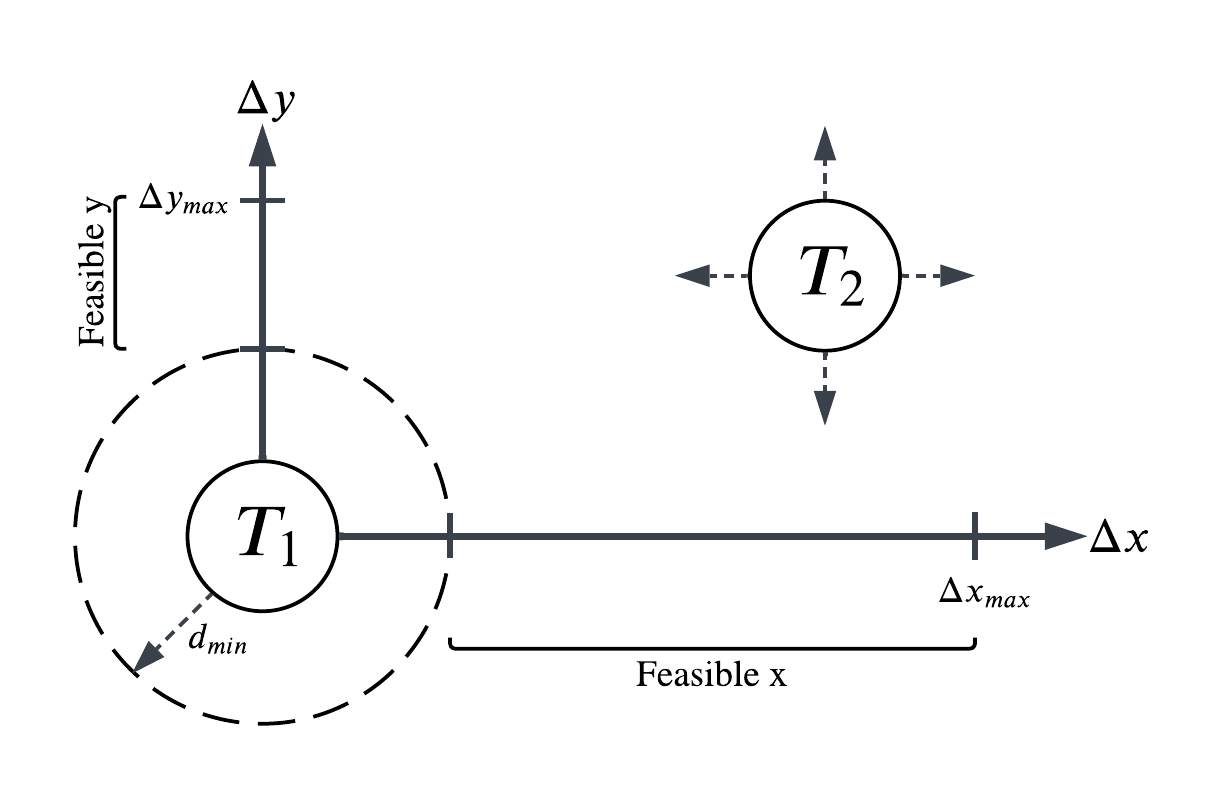
\includegraphics[width=0.6\textwidth]{figures/optimization/two_turbine_problem_schematic.png} % file name without extension
	\caption{Optimizing the relative position $\Delta x$/$\Delta y$ of a second wind turbine $T_2$ to a fixed first turbine $T_2$, constrained by minimum distance $d_{min}$ to  $T_1$ and maximum distances $\Delta x_{max}$/$\Delta y_{max}$}
	\label{fig:two_turbine_problem}
\end{figure}

The objective function to be optimized is the total power generation, e.g. the sum of power generated by both turbines. This objective is a function both of the position of the wind turbine as well as of the wind conditions like wind direction and wind speed. 

$$
f_{total Power}(x,y,\text{windspeed},\text{wind direction}, \text{(...)})
$$

Differently from the geographic coordinates, th wind condition parameters like windspeed are inherently not deterministic and follow distributions like the normal distribution as shown in Figure \ref{fig:wind_dist}.

\begin{figure}[h] 
	\centering
	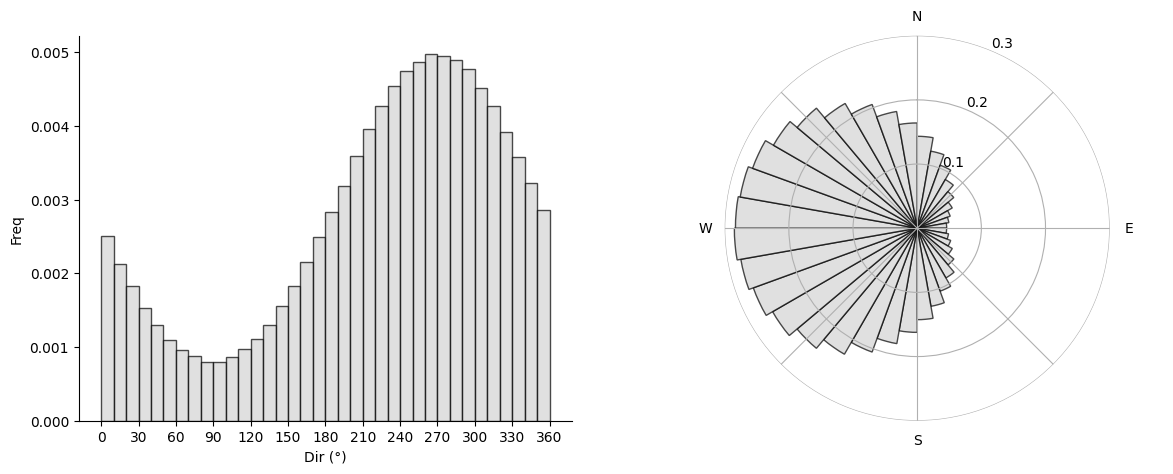
\includegraphics[width=0.9\textwidth]{figures/optimization/wind_dist.png} % file name without extension
	\caption{Histogram and Polar Plot across radiants for a normally distributed wind direction probability density function with mean West}
	\label{fig:wind_dist}
\end{figure}

The two main challenges of the optimization of the shown two turbine problem are thus: 

\begin{enumerate}
	\item Introduce the complex relationship between turbine position and wind conditions and power output into the optimization problem
	\item Introduce the non-deterministic nature of wind conditions into the optimization problem
\end{enumerate}

The first of these challenges is tackled by applying the Neural Network models discussed in Section \ref{sec:modelling} and introducing them into the optimization problem via constraint learning as described in Section \ref{sec:constraint_learning}. For the second problem, multiple approaches are now explored in the following subsection.


\subsection{Deterministic Optimization}

To begin solving the problem, the simplest approach is taken by assuming the wind conditions to be discrete. In application, this might be analogous to getting the Expectation of the joined probability distribution of all wind condition parameters. Taking these parameters as constant and homogeneous across the entire parameter space, the result is an objective function that is effectively only dependent on the relative positions of the turbine with the previously discussed geometrical constraints.

\begin{align}
	\max_{\mathbf{x}, \mathbf{y}} & f_{Power,\text{NN}}(\Delta x, \Delta y) \\
	\text{s.t.} \quad 
	&  0 \leq \Delta x \leq X_{\max} \\
	&  0 \leq \Delta y \leq Y_{\max} \\
	& \sqrt{(\Delta x)^2 + (\Delta y)^2} \geq d_{\min}
\end{align}

where:
\begin{itemize}
	\item \( (\Delta x, \Delta y) \) are the relative distances of the two turbines,
	\item \( f_{Power, \text{NN}}(\Delta x, \Delta y)\) is a neural network (deterministic) approximating the total power output ,
	\item \(  X_{\max}, Y_{\max} \) define the maximal distance the two turbines can be placed apart
	\item \( d_{\min} \) is the minimum distance between the two turbines.
\end{itemize}


\subsubsection{Modelling}

To begin with, the simulations to generate the dataset used to train the corresponding model for the deterministic case has to be generated. For the deterministic optimization, the position of the second turbine is variable in the bounds and a even steplength resulting from $n_{Steps}$ as shown in Table \ref{tab:val_determ_data}. All remaining airflow characteristics remain constant (deterministic).

\begin{table}[ht]
	\centering
	\caption{Value Ranges for Deterministic Two Turbine Problem Data Set}
	\begin{tabular}{|l|c|c|c|}
		\hline
		\textbf{Variable} & \textbf{Constant/Variable} & \textbf{Value} & \textbf{$n_{Steps}$}\\
		\hline
		$x_{\text{turb2}}$ & Variable & [0, 5000] m &\\
		$y_{\text{turb2}}$ & Variable & [0, 500] m &\\
		wind\_speed & Constant & 8 m/s & -\\
		wind\_direction & Constant & 270°&- \\
		turbulence\_intensity & Constant & 0.06 & - \\
		\hline
	\end{tabular}

	\label{tab:val_determ_data}
\end{table}

In line with the parameter space defined in Table \ref{tab:val_determ_data}, simulations are performed as described in Section \ref{sec:model_pipe}. The resulting dataset is then introduced into the Neural Network optimization method, yielding Figure \ref{fig:determ_nn_opti}. HERE WE DECIDE SOMETHING BEFORE CONtiNUING

\begin{figure}[h] 
	\centering
	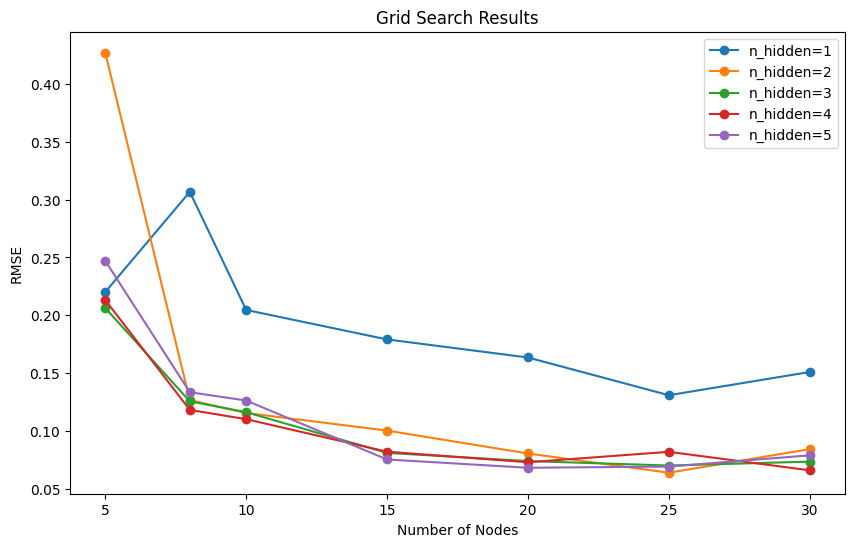
\includegraphics[width=1\textwidth]{figures/optimization/determ_nn_opti.png} 
	\caption{}
	\label{fig:determ_nn_opti}
\end{figure}

To validate the chosen model and gain a deeper understanding of its predictive power, we proceed to visualize the total power output across the variable parameter space. Figure \ref{fig:determ_model_colormap} shows a colormap generated from linealy interpolating between the datapoints for the simulation data (Subplot 1), a finder grid of predictions of the model (Subplot 2) and a colormap of the percentage deviation between model and raw data (calculated at points and then again linearly interpolated). The color in the first two subplots represents the \textit{total power generated of both wind turbines}, with the second turbine placed at the given x/y location We find that the model appears to overall represents the behaviour well, with only systematic deviation occuring at locations very close to the first wind turbine at the origin. As the simulation allows for placing wind turbines at the exact same location and with corresponding results unrealistic, simulations in this area are not necessarily correct in results either. For the optimization, the minimum distant constraint removes this area from the feasible region, meaning that the comparetively large deviations there do not affect the optimization. 

\begin{figure}[h] 
	\centering
	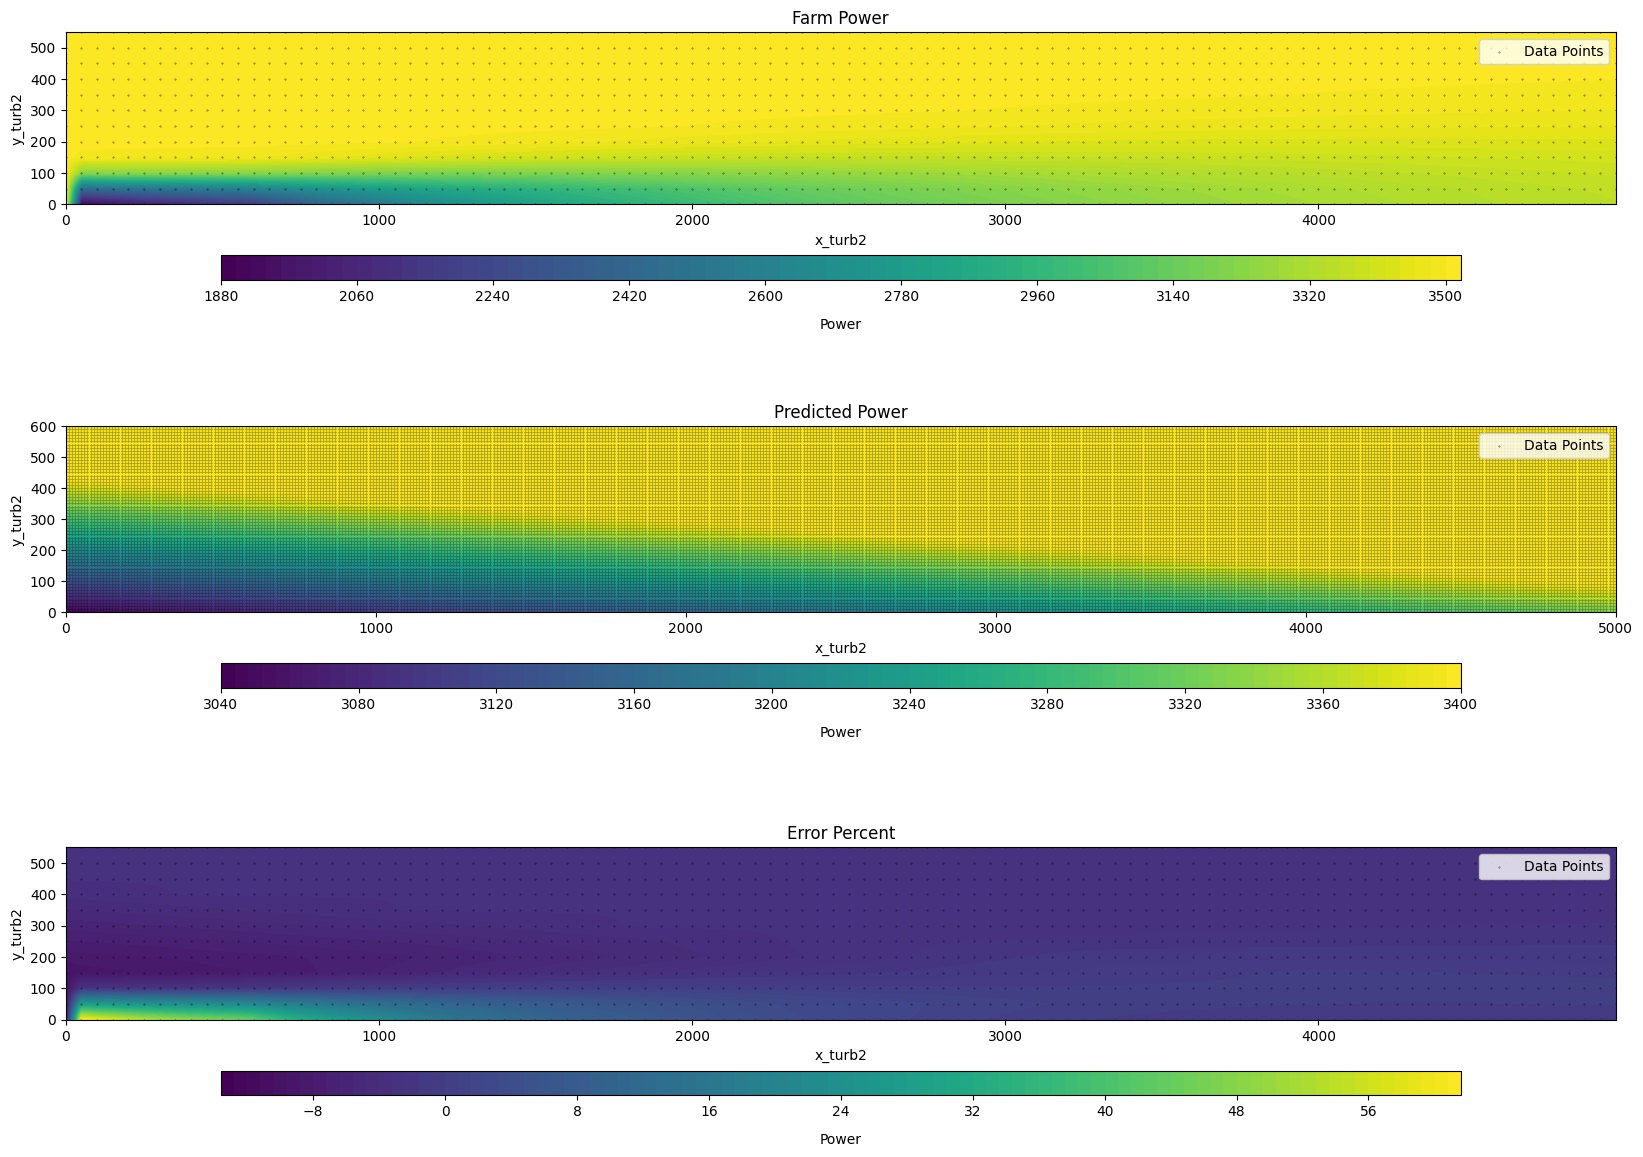
\includegraphics[width=1\textwidth]{figures/optimization/determ_model_colormap.png} 
	\caption{}
	\label{fig:determ_model_colormap}
\end{figure}

The model thus appears to be suitable to represent the interactions between the two turbines and we proceed to the optimization.

\subsubsection{Optimization}


With the model trained and validated, we proceed to implementing the defined optimization problem in pyomo  (\href{https://github.com/schmeti/uc3m_TFM_wind_farm_optimization_codebase/blob/main/Windfarm_power_modelling/0_two_turbine_problem_constrLearn_determin.ipynb}{Notebook Github}) and embedd the trained model using the the approach described in Section \ref{sec:constraint_learning}.

When solving this problem as defined using Gurobi, a major challenge becomes apparent as the result shows that there is an large number of equally optimal solutions (e.g. degeneracy of the problem, see  \cite{vanderbei2020chapter3} for an exact definition of degeneracy) everywhere outside the wake of turbine 1, as can be seen  in the visualization of the optimization result found in \ref{fig:two_turbine_heatmap_degeneracy}.


\begin{figure}[h] 
	\centering
	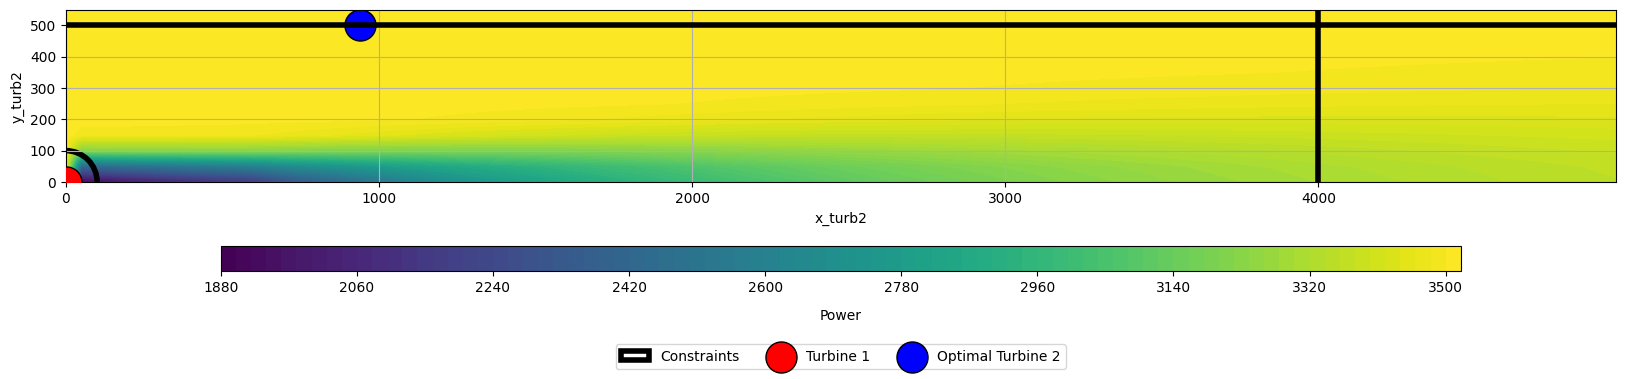
\includegraphics[width=1\textwidth]{figures/optimization/opti_determ270.png} 
	\caption{Deterministic optimization of the relative position of two windturbines relative to each other with winddirection 270° and constant windspeed}
	\label{fig:two_turbine_heatmap_degeneracy}
\end{figure}

The existence of a large number of optimal values thus has to be taken into account moving forward.


\subsection{Stochastic Optimization}

As the deterministic optimization does not take into account the distribution of wind condition parameters and having found that the deterministic approach leaves a range of infinite global optima outside of the wake of turbine 1, the next step is proceeding with the introduction of uncertainty in the form of probability distributions of wind condition parameters into the problem. To do so the objective function is modified to now represent the expected power generated by the farm, if turbine where to be placed at a given location. The Neural Network thus now has to be able to predict the power output for a given turbine 2 location taking into account the wind conditions like direction and speed at a given location. The problem is formulated as follows: 

\begin{align}
	\max_{\mathbf{x}, \mathbf{y}} &  \sum_{i=1}^{n} f_{Power,\text{NN}}(\Delta x, \Delta y, \text{wind condition})\cdot p_{n,\text{wind condtion combination}} \\
	\text{s.t.} \quad 
	&  \Delta x \leq X_{\max} \\
	&  \Delta y \leq Y_{\max} \\
	& \sqrt{(\Delta x)^2 + (\Delta y)^2} \geq d_{\min}
\end{align}

where:
\begin{itemize}
	\item \( (\Delta x, \Delta y) \) are the relative distances of the two turbines,
	\item \( f_{Power, \text{NN}}(\Delta x, \Delta y)\) is a deterministic neural network  approximating the total power output for turbine positions and wind conditions
	\item \(  X_{\max}, Y_{\max} \) define the maximal distance the two turbines can be placed apart
	\item \( d_{\min} \) is the minimum distance between the two turbines
	\item \( n \) is the index of the discretized possible combinations of wind conditions 
\end{itemize}

The following problem will first treat the univariate case of only wind direction being a random variable, with wind speed and turbolence intensity remaining constants. 

\subsubsection{Modelling}

Like for the deterministic case, we begin by finding an fitting Neural Network model to solve that can be embedded into the optimization problem. To do so, we  first again the parameter space, this time with wind direction bein variable and set up in a grid with steplength of 10°. The full parameter grid is defined in Table \ref{tab:val_prob_data}

\begin{table}[ht]
	\centering
	\caption{Value Ranges for Probabilistic Two Turbine Problem Data Set}
	\begin{tabular}{|l|c|c|c|}
		\hline
		\textbf{Variable} & \textbf{Constant/Variable} & \textbf{Value} & \textbf{$Steplength$}\\
		\hline
		$x_{\text{turb2}}$ & Variable & [0, 5000] m & 50 m\\
		$y_{\text{turb2}}$ & Variable & [0, 500] m  & 50 m\\
		wind\_speed & Constant & 8 m/s & -\\
		wind\_direction & Constant & [180°, 270°]& 10° \\
		turbulence\_intensity & Constant & 0.06 & - \\
		\hline
	\end{tabular}
	\label{tab:val_prob_data}
\end{table}

We then proceed to hyperparameter tuning of the model. Due to the added complexity, the model size has to be increased significantly to yield similarly good results compared to the deterministic case. Due to limitations in compute power, this therefore yields a reduced number of possible comparisons.


\begin{figure}[h] 
	\centering
	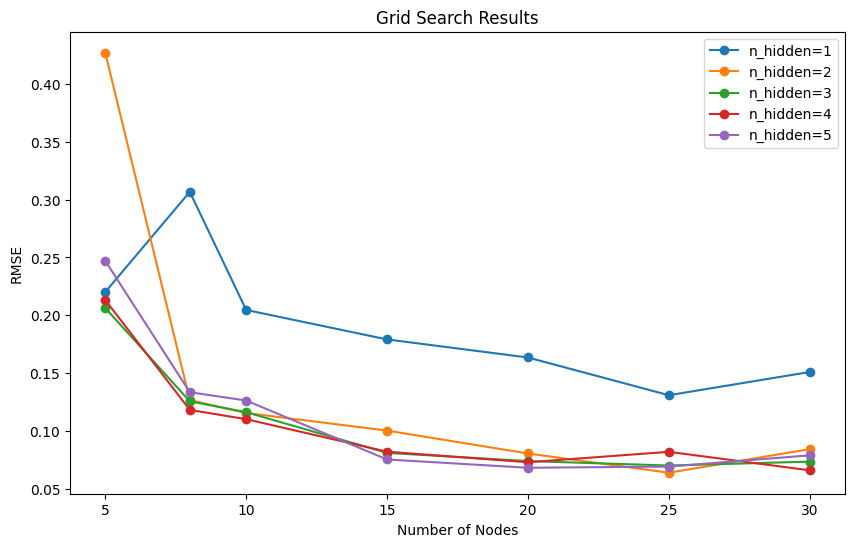
\includegraphics[width=1\textwidth]{figures/optimization/determ_nn_opti.png} 
	\caption{REPLACE FIGURE}
	\label{fig:determ_nn_opti}
\end{figure}



With a model chosen, we again performe some investigation into its performance and find that even with the significantly more complex model, the results are not as good as for the model only trained for the deterministic case. While visually the shape of the wake generally appears to fit, the deviation in percent shows are more farreaching deviation, even at greater distances away from Turbine 1, as can be seen in Figure \ref{fig:prob_model_colormap} for wind direction 260° . 

\begin{figure}[h] 
	\centering
	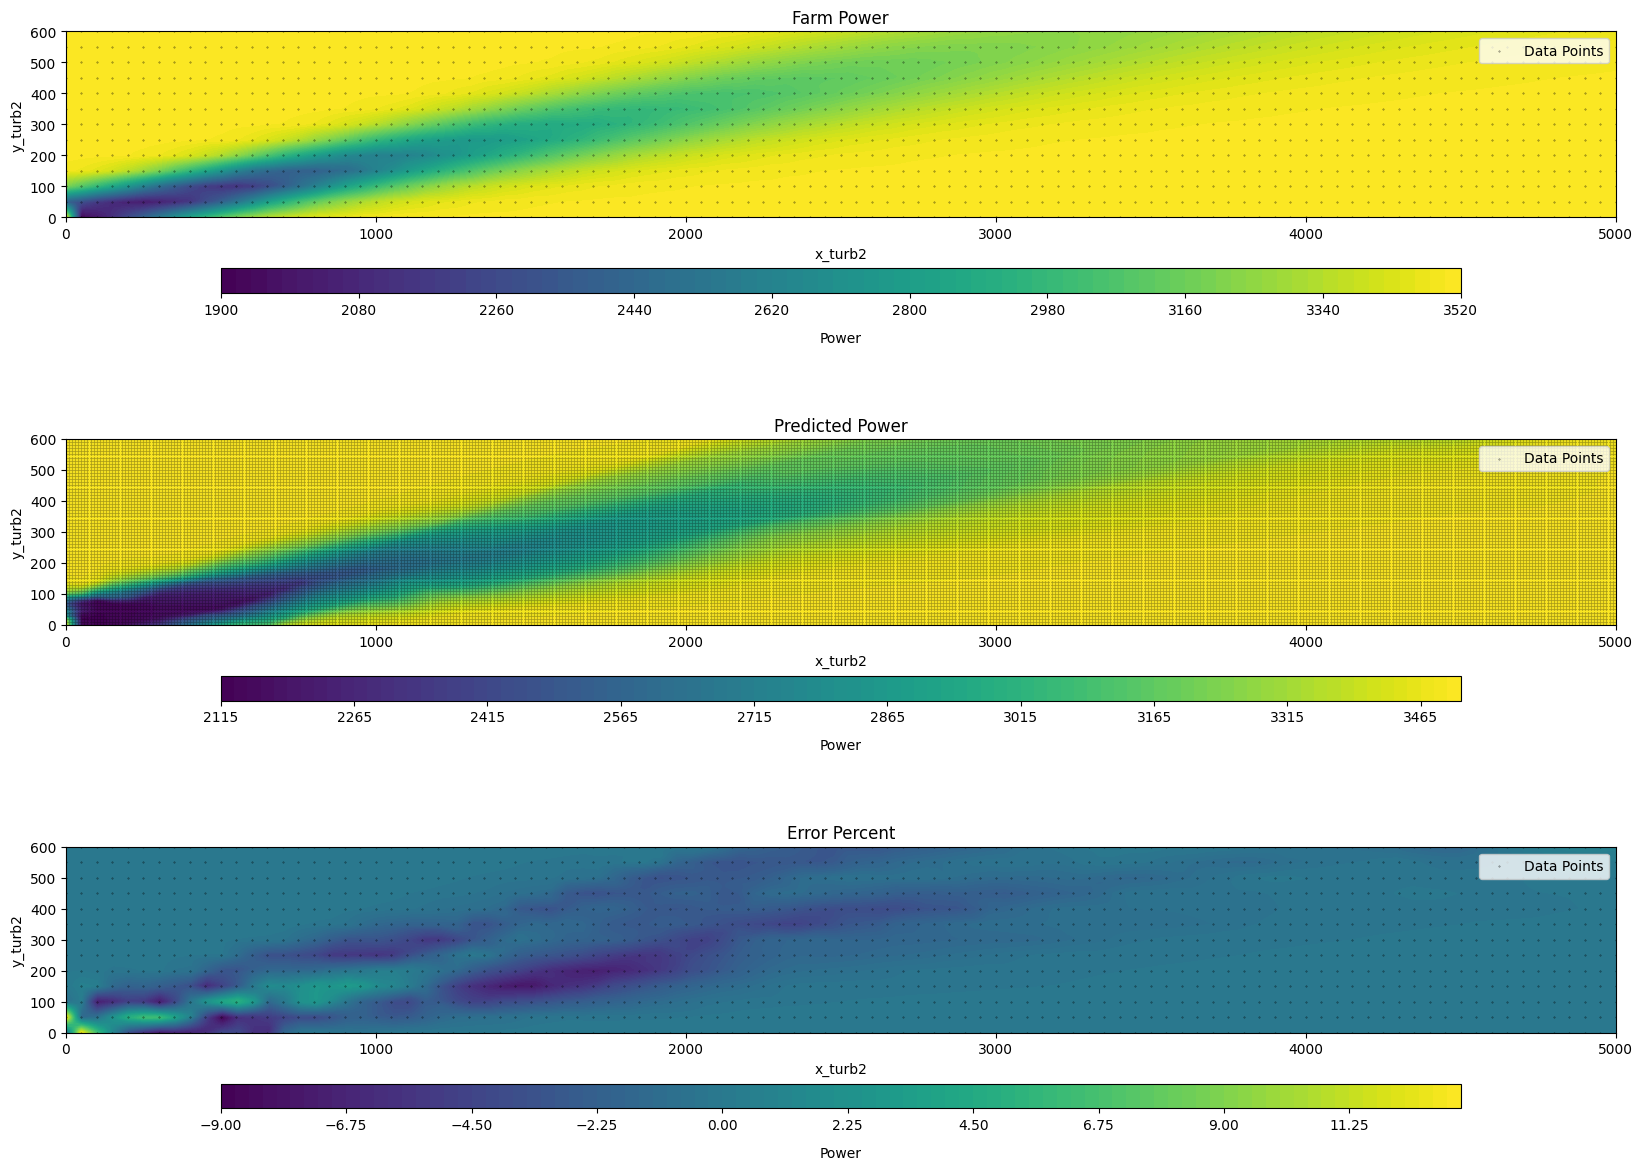
\includegraphics[width=1\textwidth]{figures/optimization/prob_model_colormap.png} 
	\caption{A heatmap of total generated farm power for a winddirection of 260° with datapoints and linear interpolation inbetween. Plot 1 shows the raw data, plot 2 the predictions of the $\text{NN}(5\,{-}\,25^{\times10}\,{-}\,1)$, plot 3 the percentage difference between training points and predictions }
	\label{fig:prob_model_colormap}
\end{figure}

Since the parameter space has now become three dimensional, conditioning on a single winddirection does not cover the full performance of the model. Figure \ref{label} therefore shows the development of RMSE across different winddirection, indicating that the border regions and wind directions with an increased total wake lenght (e.g. wind directions closer to 270° wind direction) experience higher RMSE. 

\begin{figure}[h] 
	\centering
	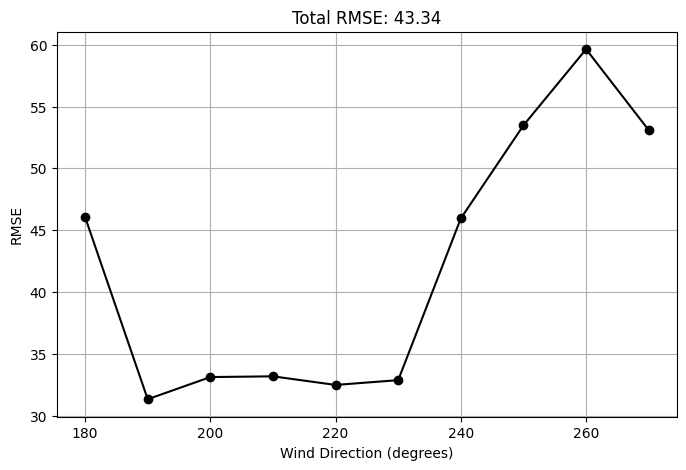
\includegraphics[width=0.6\textwidth]{figures/optimization/rmse_dist_10layers25nodes.png}
	\caption{RMSE of  $\text{NN}(5\,{-}\,25^{\times10}\,{-}\,1)$ across the parameter space of wind direction }
	\label{fig:rmse_dist_10layers25nodes}
\end{figure}


For optimization purposes, the individual power per wind direction however becomes less relevant, as the power outputs are weighted by their probability of occouring. 
To do so, we first have to define the probability distribution of the wind directions. For simplicity sake, a Normal distribution with mean 270° and standard deviation of 5°, as shown in Figure \ref{fig:wind_dist_opti}.


\begin{figure}[h] 
	\centering
	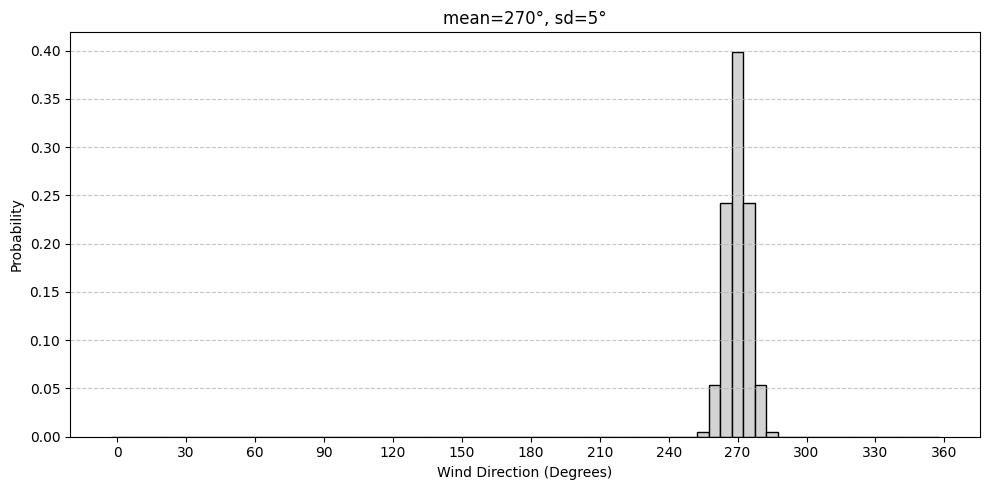
\includegraphics[width=0.8\textwidth]{figures/optimization/wind_dist_opti.png} 
	\caption{Discrete Wind Direction Probability Distribution with mean 270° and standard deviation 5°, discretized in intervals of 10° }
	\label{fig:wind_dist_opti}
\end{figure}


Using this distribution, the expected power for the ranges of x and y coordinates can thus now be calculated by aggregating the powers for the different wind directions as a sum weighted by probability to yield the expected farm power generated at the specific coordinate. By evaluating the expected farm power both for the training data as well as for predictions for the training data, we can again compare the results and deviations as done in Figure \ref{label} 

\begin{figure}[h] 
	\centering
	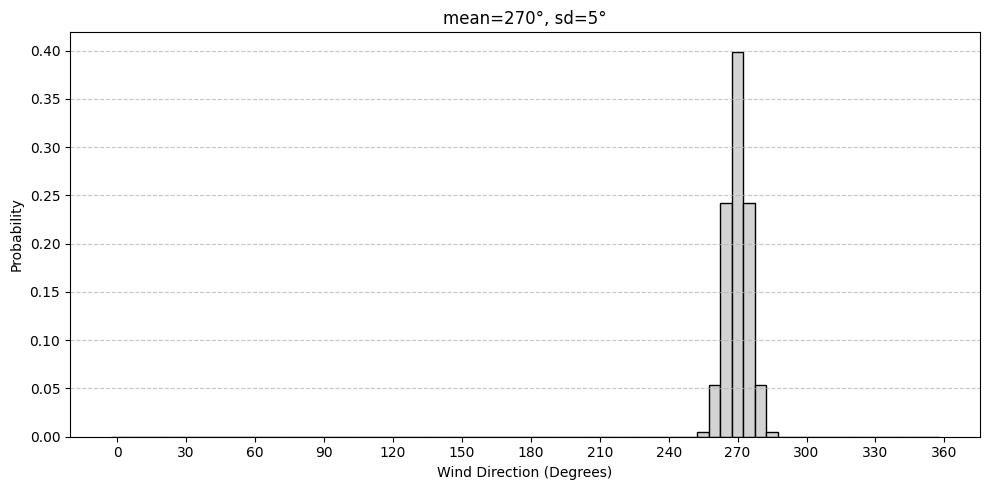
\includegraphics[width=0.8\textwidth]{figures/optimization/wind_dist_opti.png} 
	\caption{REPLACE FIGURE }
	\label{fig:wind_dist_opti}
\end{figure}



While increasing the size of the Neural Network would undoubtetly reduce the deviations across wind directions and for the individual wind directions, the size of the Neural Network is restricted by the solvability of the optimization problem. While there is no exact threshold, solving time of the mixed integer problem that results from the embedding of the Neural Network increases roughly exponentially by adding Neurons to the Network and therefore adding binary variables to the problem. The shown Neural Network was thus found to be the maximum feasible size of Neural Network for the given computational recourses. 


The same way the distribution of farm power was previously dependent on the wind direction, it is now dependent on the wind direction distribution and therefore in the case of the Normal, on its mean and variance. Changing the mean of the distribution corresponds to changing the direction of the principal wind direction and thus the direction of the highest expected wake losses from turbine 1. Meanwhile, increasing the variance corresponds to spreading the expected wake losses due to turbine 1 across a wider range of wind directions and therefore increasing the areaaffected by expected wake losses, while reducing the absolute reduction in expected power within the area affected by the wake. This relationship can be seen in the expected power distribution for a normal with mean MEAN and standard deviation STDEVIATION shown in Figure \ref{label}


\begin{figure}[h] 
	\centering
	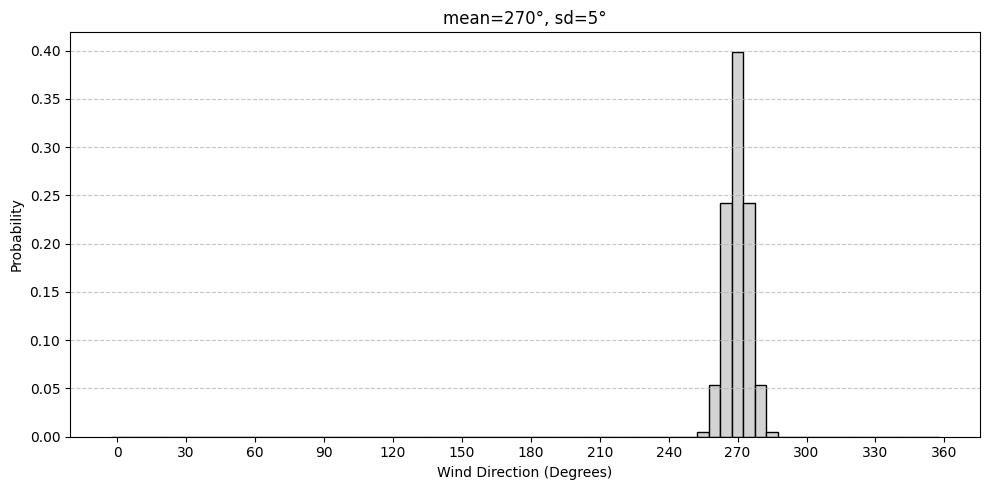
\includegraphics[width=0.8\textwidth]{figures/optimization/wind_dist_opti.png} 
	\caption{REPLACE FIGURE }
	\label{fig:wind_dist_opti}
\end{figure}


The normal distribution is used in this thesis as a placeholder for proof of concept purposes. In practice, in practical application, the real wind distribution would have to be evaluated at the specific location. 

TODO: Improvements -> train NN slightly beyondactual parameter space

\subsubsection{Optimization}

With the model set up, solving the stochastich optimization problem for a maximial expected farm power output can be attempted

The Neural Network and the wind direction distribution is  again introduced into pyomo to find a global maximum. Like before, plotting the result as shown in \ref{fig:prob_data_lininter}, it is possible to visually find that there is a large range of more or less equally optimal points in the wind directions that the wind distribution discretization does not cover the space evenly as the parameter space for x and y of turbine 2 are not identical. The discretization in the shown scenarios thus does not sufficiently cover the whole space, leading to seemingly optimal areas where in reality significant wake losses can be expected.


\begin{figure}[h] 
	\centering
	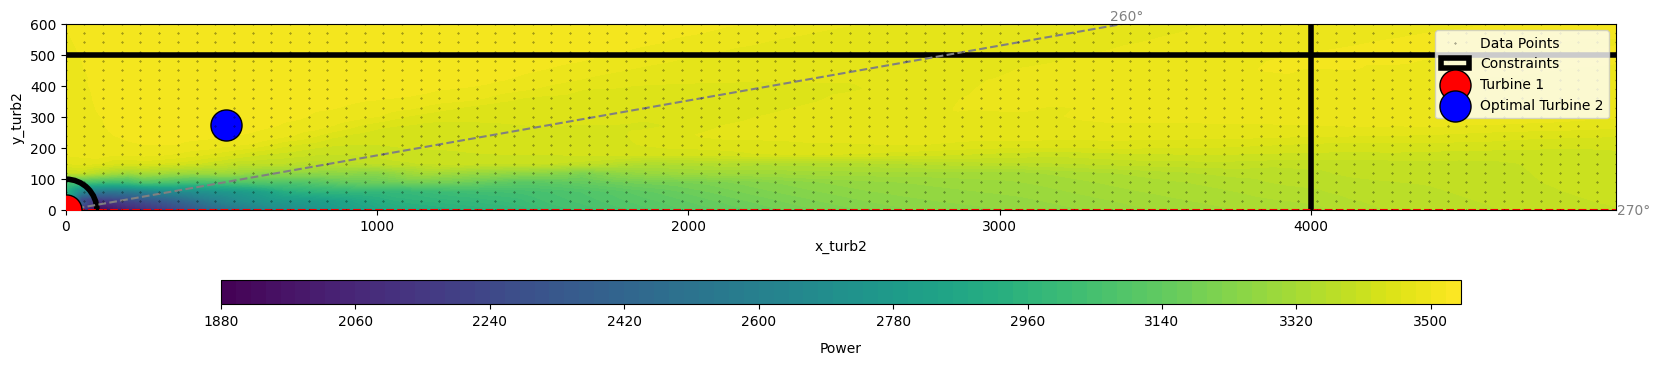
\includegraphics[width=1\textwidth]{figures/optimization/prob_data_lininter.png} 
	\caption{}
	\label{fig:prob_data_lininter}
\end{figure}

In practice, the size of the Neural Network required to represent the farm power function makes the identification of the global optimum challanging due to the number of integer variables added to the problem. Adding to this is the large range of nearly equal optimal solutions, leading to solvers like gurobi to require extremely large runtimes. The development of best optimal and upper limit, showing how the maximum of the objective function remains nearly identical, the upper limit to the solution converges towards the first found optima. This behaviour can bee seend in Figure \ref{asd}

\begin{figure}[h] 
	\centering
	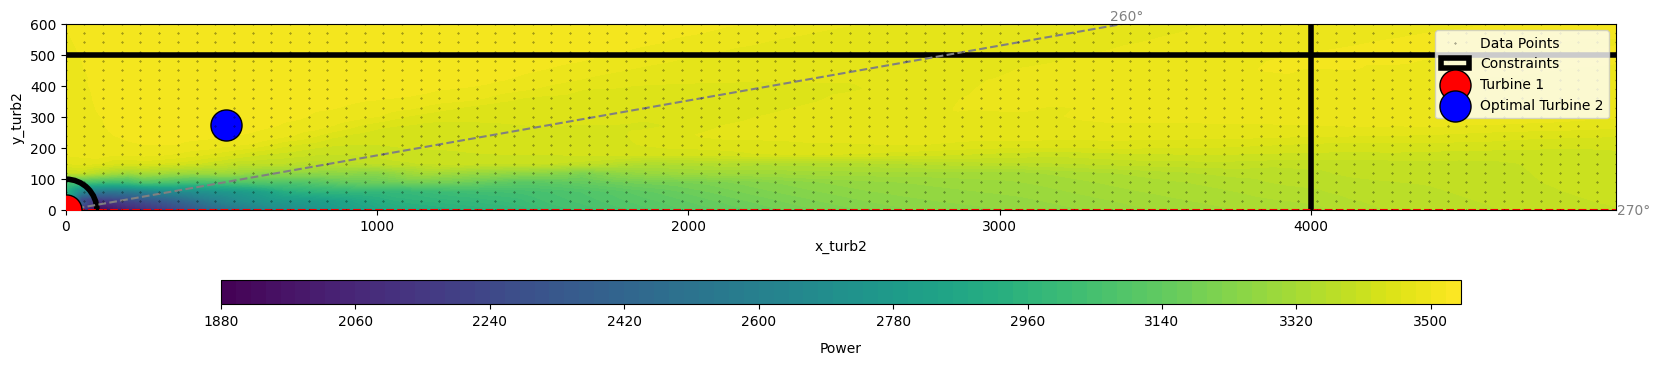
\includegraphics[width=1\textwidth]{figures/optimization/prob_data_lininter.png} 
	\caption{}
	\label{fig:prob_data_lininter}
\end{figure} 

TODO : PLAY WITH CONSTRAINTS

A discussion of the value of this approach will be performed in the conclusion of this thesis. 
	
\subsubsection{Stochastic Optimization: Quantile Discretization of Wind Direction Distribution }

One thing noticable in the previously shown plots of the distribution of theexpected farm power is how it is affected by the discretization of the wind directions, previously done in 10° steps. This does however mean that in the directions for which a long wake is considered (x direction/ 270°) the space in between the space between the scenarios  is fairly large, as very apparent  by the degree lines shwon in the solution to the probabilistic case (Figure \ref{label}). A way to take this into account is by discretizing not with an constant step length but based on the quantiles of the distribution. The discretization can thus be performed not by a constant length of the disrcetization steps, but a constant probability within a chosen number of quantiles. For each quantile individually the mean is then calculated and the resulting expected values for the quantile are taken as discretization steps. Such an approach used for the same Normal distribution with mean 270° and standard deviation 5° degrees, fixing the scenario/quantile count to 7, yields the discretization shown in Figure \ref{fig:wind_dist_opti_quantiles}. 

\begin{figure}[h] 
	\centering
	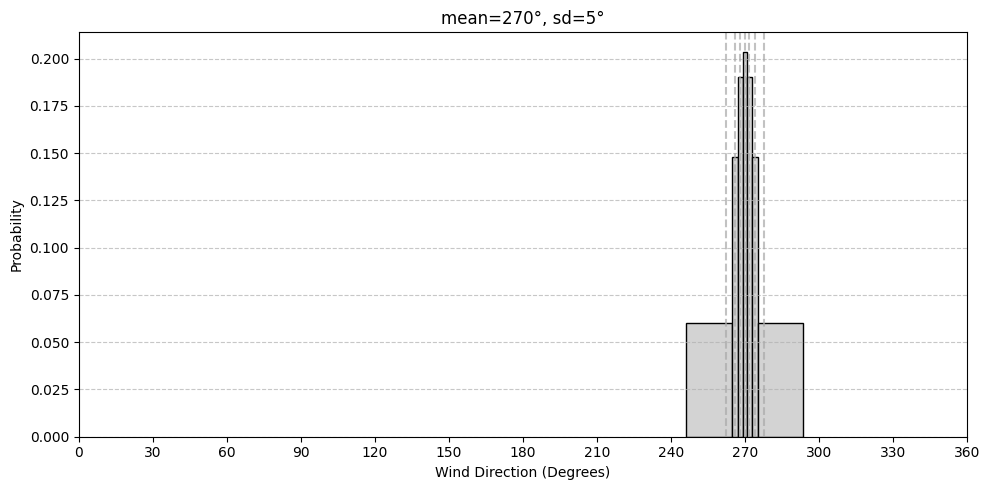
\includegraphics[width=0.8\textwidth]{figures/optimization/wind_dist_opti_quantiles.png} 
	\caption{Quantile based discretization of Normal mean 270°,  standard deviation 5°, disrcetized into 7 scenarios with equal probability for scenario and the scenario angle corresponding to the expected value for the quantile }
	\label{fig:wind_dist_opti_quantiles}
\end{figure} 

Using this distribution, the expected power distribution changes for the corresponding scenarios/quantiles, with the the expected wake losses moving towards the true high-probability zone for wake losses. The optimal area thus moves out of the spaces inbetween scenarios to the true zone of low expected wake losses, as can be seen in Figure \ref{label}

\subsubsection{Stochastic Optimization: Unsymmetric Wind Direction Distributions}


\section{The three Turbine Problem}

\section{The n Turbine Problem}

Thoughts: 

IDEA: generalize inputs in a way that allow for power calculation of each turbine individually instead of farm power

IDEA : derive basic rules from 2 turbine problem and set up new optimization problem without NN 

IDEA : analogue to forward/backward selection with 2 turbine neural network


FINIDINGS: 

problem degenerate if not one wind turbine fixed

\section{Possible Improvements in Optimization}

The main limitation of the approach as presented in this chapter is that the increasing the number of neurons in the Neural Network by one neuron increases the number of integer variables by one and the number of constraints by three, while adding an additional scenario requires reintroducing the entire Neural Network for that specific scenario. As computation time is a function of the number of constraints and decision variables, the computation time increases approximately exponentially with adding neurons or scenarios. 

Finding a way to reduce the number of constraints/integer variables would thus be the main concern when attempting to improve the presented method. 